\section{Modelo entidad relación:}

\begin{figure}[H]
  \centering
  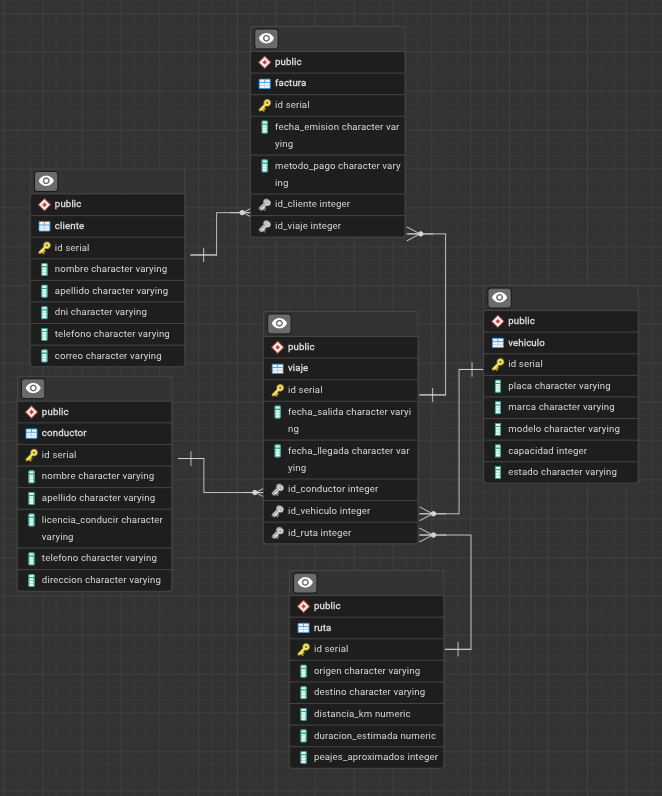
\includegraphics[width=1\textwidth]{assets/mer.png}
\end{figure}

\newpage

\section{Creación de la base de datos y tablas:}
  \begin{itemize}
    \item
      \begin{figure}[H]
        \centering
        
\includegraphics[width=1\textwidth]{assets/a1.png}
      \end{figure}
    \begin{figure}[H]
      \centering
      
\includegraphics[width=1\textwidth]{assets/a2.png}
      \caption{Conductor}
    \end{figure}
    \begin{figure}[H]
      \centering
      
\includegraphics[width=1\textwidth]{assets/a3.png}
      \caption{Vehículo}
    \end{figure}
    \begin{figure}[H]
      \centering
      
\includegraphics[width=1\textwidth]{assets/a4.png}
      \caption{Ruta}
    \end{figure}
    \begin{figure}[H]
      \centering
      
\includegraphics[width=1\textwidth]{assets/a5.png}
      \caption{Cliente}
    \end{figure}
    \begin{figure}[H]
      \centering
      
\includegraphics[width=1\textwidth]{assets/a6.png}
      \caption{Viaje}
    \end{figure}
    \begin{figure}[H]
      \centering
      
\includegraphics[width=1\textwidth]{assets/a7.png}
      \caption{Factura}
    \end{figure}
  \end{itemize}

\section{Poblado de la base de datos}

\begin{itemize}
  \item
    \begin{figure}[H]
      \centering
      
\includegraphics[width=1\textwidth]{assets/b1.png}
      \caption{Conductor}
    \end{figure}
    \begin{figure}[H]
      \centering
      
\includegraphics[width=1\textwidth]{assets/b2.png}
      \caption{Vehículo}
    \end{figure}
    \begin{figure}[H]
      \centering
      
\includegraphics[width=1\textwidth]{assets/b3.png}
      \caption{Ruta}
    \end{figure}
    \begin{figure}[H]
      \centering
      
\includegraphics[width=1\textwidth]{assets/b4.png}
      \caption{Cliente}
    \end{figure}
    \begin{figure}[H]
      \centering
      
\includegraphics[width=1\textwidth]{assets/b5.png}
      \caption{Viaje}
    \end{figure}
    \begin{figure}[H]
      \centering
      
\includegraphics[width=1\textwidth]{assets/b6.png}
      \caption{Factura}
    \end{figure}
  \end{itemize}

  \newpage

  \section{Muestra de consultas SQL:}
  \begin{itemize}
    \item
      \begin{figure}[H]
        \centering
        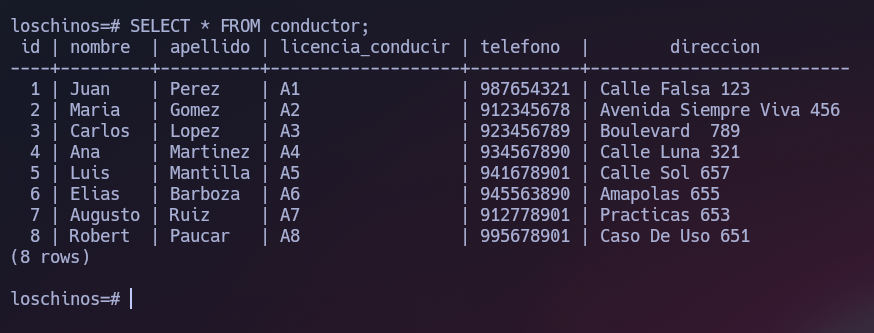
\includegraphics[width=1\textwidth]{assets/c1.png}
        \caption{Consulta 1: Conductores}
      \end{figure}
      \begin{figure}[H]
        \centering
        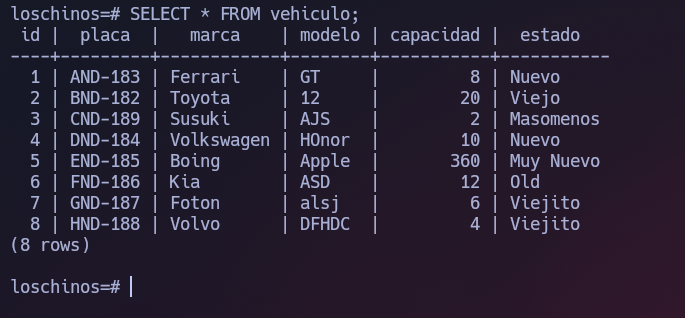
\includegraphics[width=1\textwidth]{assets/c2.png}
        \caption{Consulta 2: Vehículos}
      \end{figure}
      \begin{figure}[H]
        \centering
        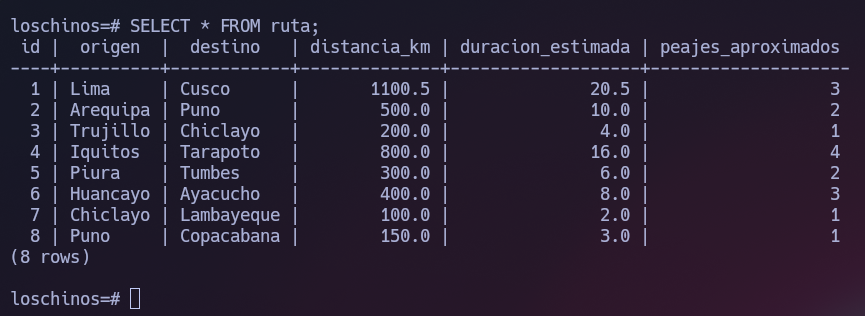
\includegraphics[width=1\textwidth]{assets/c3.png}
        \caption{Consulta 3: Rutas}
      \end{figure}
      \begin{figure}[H]
        \centering
        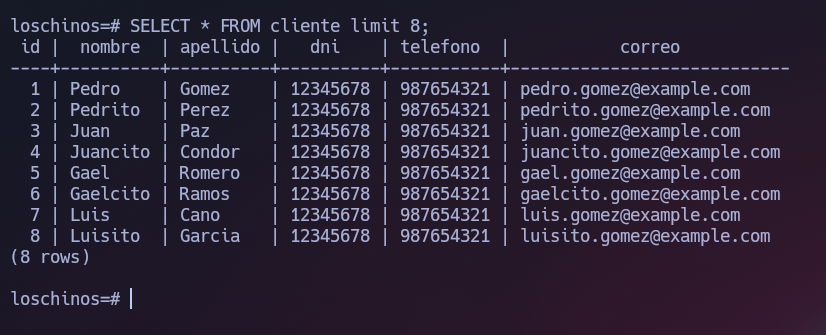
\includegraphics[width=1\textwidth]{assets/c4.png}
        \caption{Consulta 4: Clientes}
      \end{figure}
      \begin{figure}[H]
        \centering
        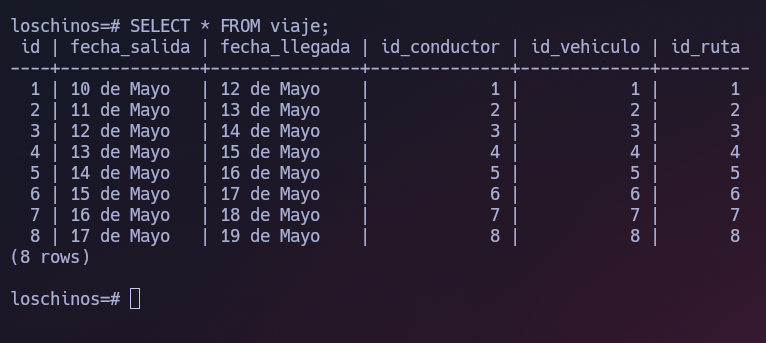
\includegraphics[width=1\textwidth]{assets/c5.png}
        \caption{Consulta 5: Viajes}
      \end{figure}
      \begin{figure}[H]
        \centering
        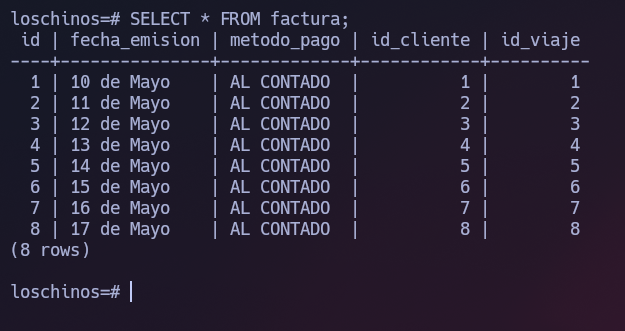
\includegraphics[width=1\textwidth]{assets/c6.png}
        \caption{Consulta 6: Facturas}
      \end{figure}
  \end{itemize}

  \newpage

  \section{Diagrama de Caso de Uso}

  \begin{figure}[H]
    \centering
    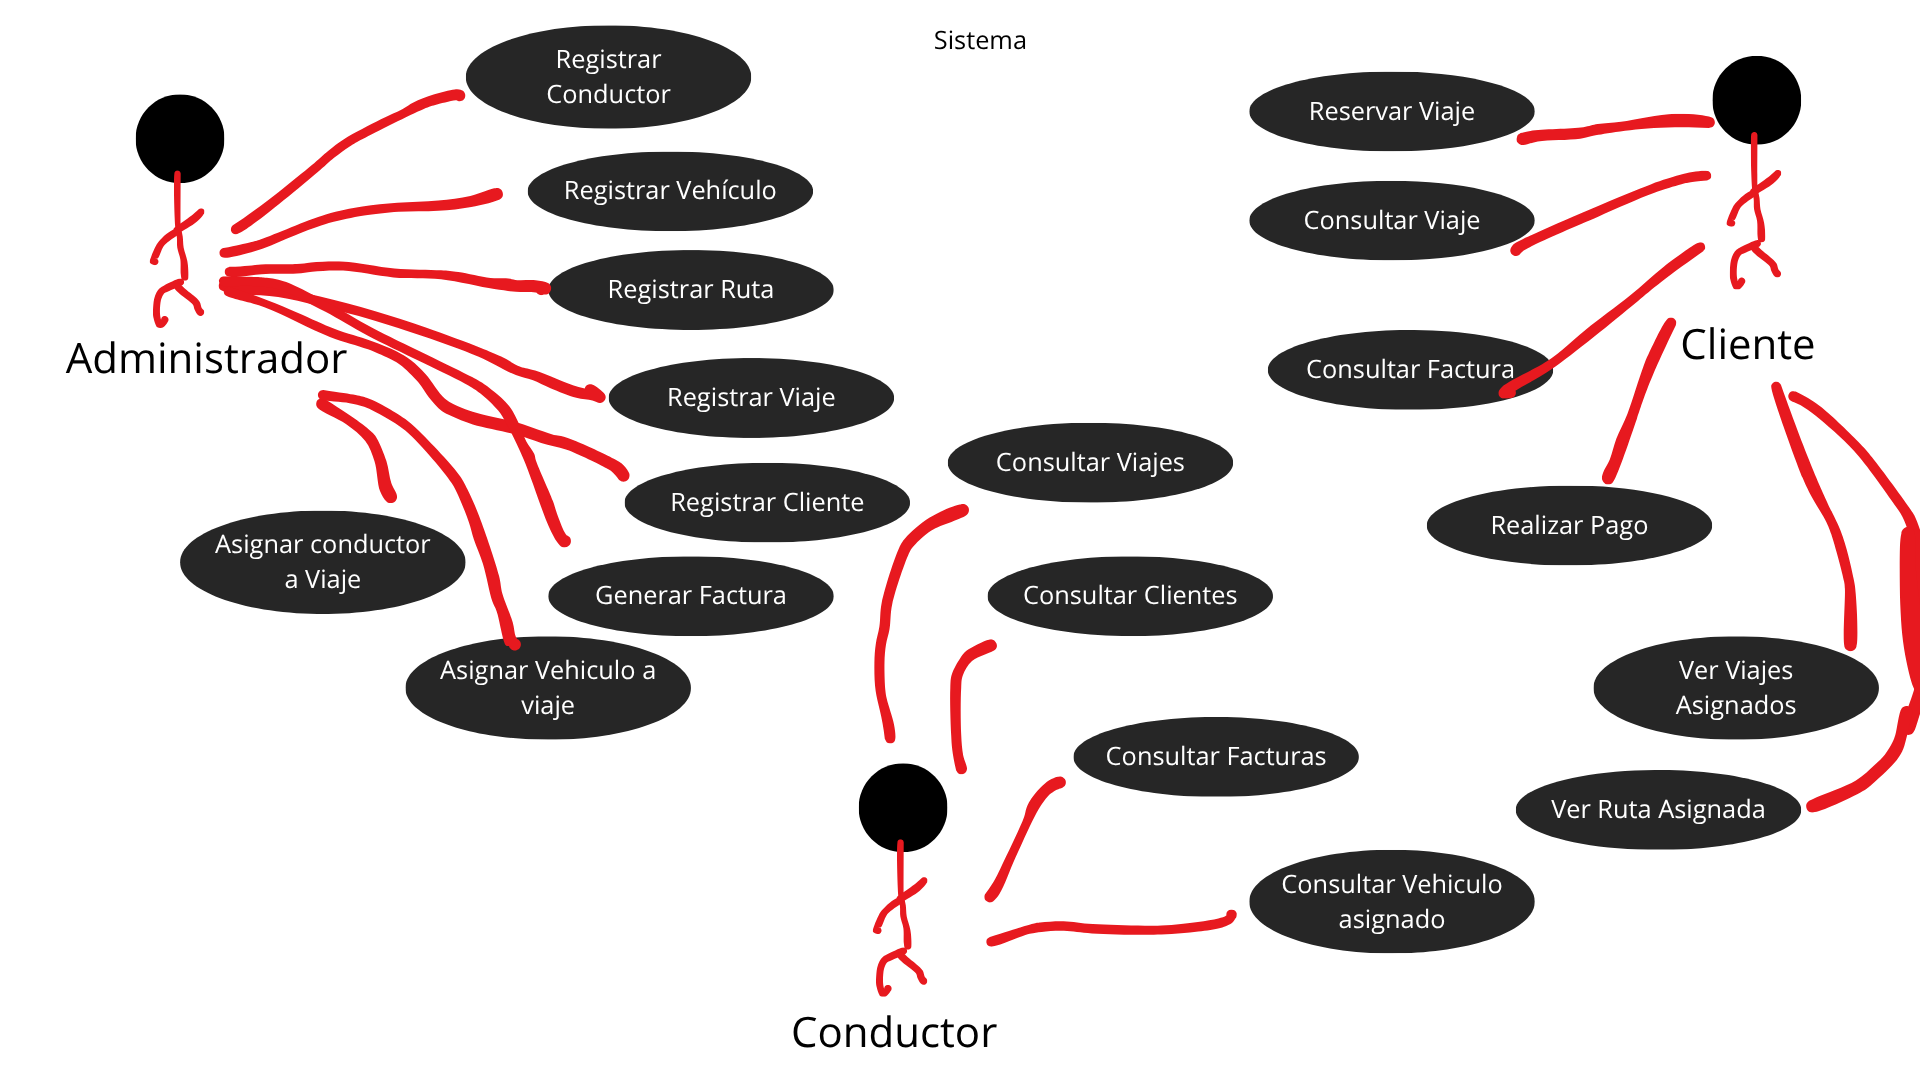
\includegraphics[width=1\textwidth]{assets/dcu.png}
    \caption{Diagrama de Caso de Uso}
  \end{figure}
\newpage
  \section{Requerimientos}

  \textbf{Según:}

  \textit{Mostrar la lista de conductores con sus nombres, apellidos, licencias de conducir ordenados por apellidos en forma ascendente. }

  \begin{figure}[H]
    \centering
    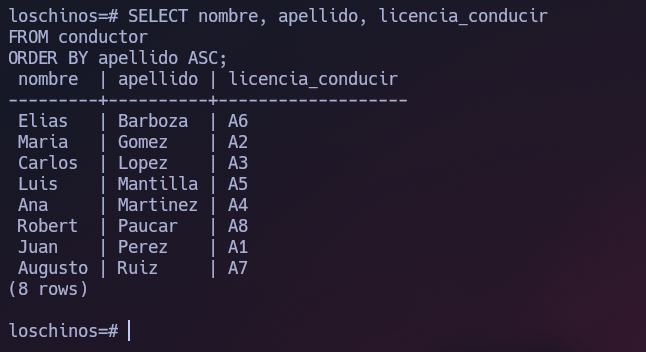
\includegraphics[width=1\textwidth]{assets/e1.png}
    \caption{Requerimiento 1}
  \end{figure}


    \textit{Mostrar la lista de los 3 primeros vehículos mostrando su placa, marca, modelo y capacidad. }

    \begin{figure}[H]
    \centering
    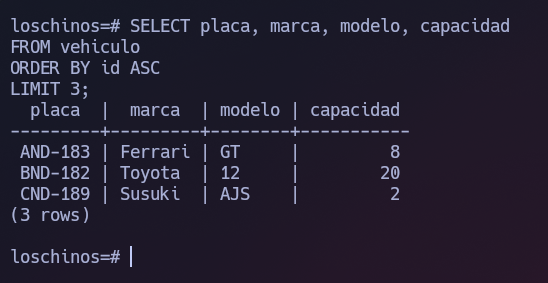
\includegraphics[width=1\textwidth]{assets/e2.png}
    \caption{Requerimiento 2}
  \end{figure}

  \newpage

\textbf{Finalmente:}

  \textit{Profesor, me parece extraño que no haya dejado nada de combinaciones/joins por lo que para evitarme dolores de cabeza le dejo uno por si acaso.}

  Se muestra el nombre del conductor con la fecha de salida y llegada del viaje asignado.

    \begin{figure}[H]
    \centering
    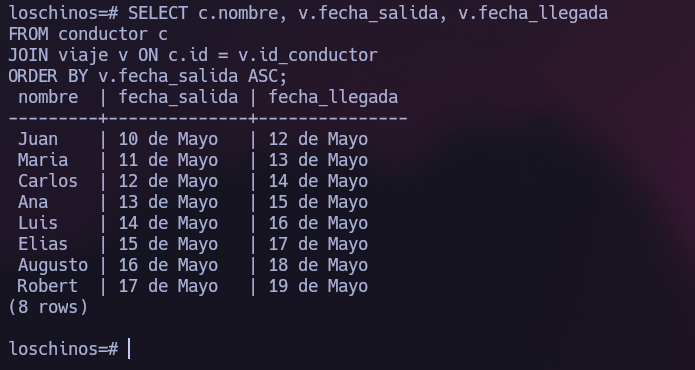
\includegraphics[width=1\textwidth]{assets/E3.png}
    \caption{Mi join}
  \end{figure}
